% Created by tikzDevice version 0.12.6 on 2024-08-18 22:25:33
% !TEX encoding = UTF-8 Unicode
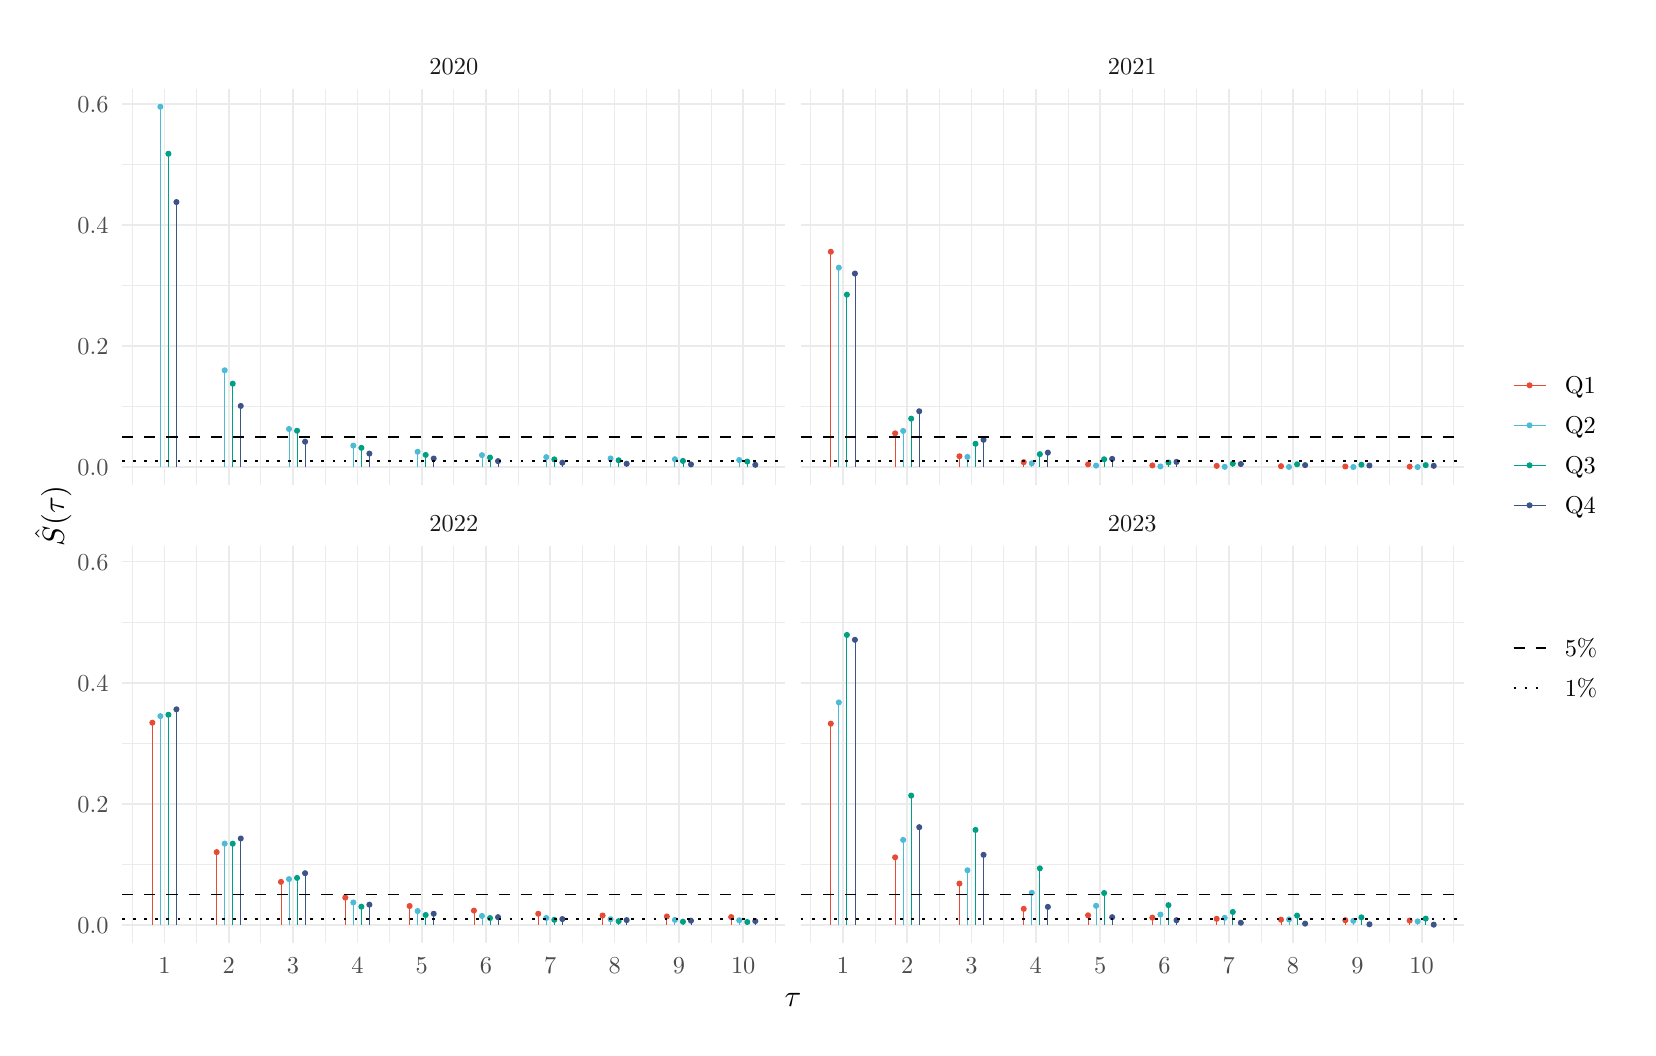
\begin{tikzpicture}[x=1pt,y=1pt]
\definecolor{fillColor}{RGB}{255,255,255}
\path[use as bounding box,fill=fillColor,fill opacity=0.00] (0,0) rectangle (578.16,361.35);
\begin{scope}
\path[clip] ( 34.16,196.02) rectangle (273.82,339.28);
\definecolor{drawColor}{gray}{0.92}

\path[draw=drawColor,line width= 0.3pt,line join=round] ( 34.16,224.39) --
	(273.82,224.39);

\path[draw=drawColor,line width= 0.3pt,line join=round] ( 34.16,268.12) --
	(273.82,268.12);

\path[draw=drawColor,line width= 0.3pt,line join=round] ( 34.16,311.85) --
	(273.82,311.85);

\path[draw=drawColor,line width= 0.3pt,line join=round] ( 37.79,196.02) --
	( 37.79,339.28);

\path[draw=drawColor,line width= 0.3pt,line join=round] ( 61.03,196.02) --
	( 61.03,339.28);

\path[draw=drawColor,line width= 0.3pt,line join=round] ( 84.27,196.02) --
	( 84.27,339.28);

\path[draw=drawColor,line width= 0.3pt,line join=round] (107.51,196.02) --
	(107.51,339.28);

\path[draw=drawColor,line width= 0.3pt,line join=round] (130.75,196.02) --
	(130.75,339.28);

\path[draw=drawColor,line width= 0.3pt,line join=round] (153.99,196.02) --
	(153.99,339.28);

\path[draw=drawColor,line width= 0.3pt,line join=round] (177.23,196.02) --
	(177.23,339.28);

\path[draw=drawColor,line width= 0.3pt,line join=round] (200.47,196.02) --
	(200.47,339.28);

\path[draw=drawColor,line width= 0.3pt,line join=round] (223.71,196.02) --
	(223.71,339.28);

\path[draw=drawColor,line width= 0.3pt,line join=round] (246.94,196.02) --
	(246.94,339.28);

\path[draw=drawColor,line width= 0.3pt,line join=round] (270.18,196.02) --
	(270.18,339.28);

\path[draw=drawColor,line width= 0.6pt,line join=round] ( 34.16,202.53) --
	(273.82,202.53);

\path[draw=drawColor,line width= 0.6pt,line join=round] ( 34.16,246.26) --
	(273.82,246.26);

\path[draw=drawColor,line width= 0.6pt,line join=round] ( 34.16,289.99) --
	(273.82,289.99);

\path[draw=drawColor,line width= 0.6pt,line join=round] ( 34.16,333.72) --
	(273.82,333.72);

\path[draw=drawColor,line width= 0.6pt,line join=round] ( 49.41,196.02) --
	( 49.41,339.28);

\path[draw=drawColor,line width= 0.6pt,line join=round] ( 72.65,196.02) --
	( 72.65,339.28);

\path[draw=drawColor,line width= 0.6pt,line join=round] ( 95.89,196.02) --
	( 95.89,339.28);

\path[draw=drawColor,line width= 0.6pt,line join=round] (119.13,196.02) --
	(119.13,339.28);

\path[draw=drawColor,line width= 0.6pt,line join=round] (142.37,196.02) --
	(142.37,339.28);

\path[draw=drawColor,line width= 0.6pt,line join=round] (165.61,196.02) --
	(165.61,339.28);

\path[draw=drawColor,line width= 0.6pt,line join=round] (188.85,196.02) --
	(188.85,339.28);

\path[draw=drawColor,line width= 0.6pt,line join=round] (212.09,196.02) --
	(212.09,339.28);

\path[draw=drawColor,line width= 0.6pt,line join=round] (235.32,196.02) --
	(235.32,339.28);

\path[draw=drawColor,line width= 0.6pt,line join=round] (258.56,196.02) --
	(258.56,339.28);
\definecolor{drawColor}{RGB}{77,187,213}
\definecolor{fillColor}{RGB}{77,187,213}

\path[draw=drawColor,line width= 0.4pt,line join=round,line cap=round,fill=fillColor] ( 47.95,332.77) circle (  0.89);

\path[draw=drawColor,line width= 0.4pt,line join=round,line cap=round,fill=fillColor] ( 71.19,237.54) circle (  0.89);

\path[draw=drawColor,line width= 0.4pt,line join=round,line cap=round,fill=fillColor] ( 94.43,216.33) circle (  0.89);

\path[draw=drawColor,line width= 0.4pt,line join=round,line cap=round,fill=fillColor] (117.67,210.33) circle (  0.89);

\path[draw=drawColor,line width= 0.4pt,line join=round,line cap=round,fill=fillColor] (140.91,208.11) circle (  0.89);

\path[draw=drawColor,line width= 0.4pt,line join=round,line cap=round,fill=fillColor] (164.15,206.87) circle (  0.89);

\path[draw=drawColor,line width= 0.4pt,line join=round,line cap=round,fill=fillColor] (187.39,206.16) circle (  0.89);

\path[draw=drawColor,line width= 0.4pt,line join=round,line cap=round,fill=fillColor] (210.63,205.68) circle (  0.89);

\path[draw=drawColor,line width= 0.4pt,line join=round,line cap=round,fill=fillColor] (233.87,205.41) circle (  0.89);

\path[draw=drawColor,line width= 0.4pt,line join=round,line cap=round,fill=fillColor] (257.11,205.12) circle (  0.89);
\definecolor{drawColor}{RGB}{0,160,135}
\definecolor{fillColor}{RGB}{0,160,135}

\path[draw=drawColor,line width= 0.4pt,line join=round,line cap=round,fill=fillColor] ( 50.86,315.79) circle (  0.89);

\path[draw=drawColor,line width= 0.4pt,line join=round,line cap=round,fill=fillColor] ( 74.10,232.70) circle (  0.89);

\path[draw=drawColor,line width= 0.4pt,line join=round,line cap=round,fill=fillColor] ( 97.34,215.70) circle (  0.89);

\path[draw=drawColor,line width= 0.4pt,line join=round,line cap=round,fill=fillColor] (120.58,209.52) circle (  0.89);

\path[draw=drawColor,line width= 0.4pt,line join=round,line cap=round,fill=fillColor] (143.82,206.96) circle (  0.89);

\path[draw=drawColor,line width= 0.4pt,line join=round,line cap=round,fill=fillColor] (167.06,206.02) circle (  0.89);

\path[draw=drawColor,line width= 0.4pt,line join=round,line cap=round,fill=fillColor] (190.30,205.35) circle (  0.89);

\path[draw=drawColor,line width= 0.4pt,line join=round,line cap=round,fill=fillColor] (213.54,205.02) circle (  0.89);

\path[draw=drawColor,line width= 0.4pt,line join=round,line cap=round,fill=fillColor] (236.78,204.80) circle (  0.89);

\path[draw=drawColor,line width= 0.4pt,line join=round,line cap=round,fill=fillColor] (260.02,204.57) circle (  0.89);
\definecolor{drawColor}{RGB}{60,84,136}
\definecolor{fillColor}{RGB}{60,84,136}

\path[draw=drawColor,line width= 0.4pt,line join=round,line cap=round,fill=fillColor] ( 53.76,298.34) circle (  0.89);

\path[draw=drawColor,line width= 0.4pt,line join=round,line cap=round,fill=fillColor] ( 77.00,224.66) circle (  0.89);

\path[draw=drawColor,line width= 0.4pt,line join=round,line cap=round,fill=fillColor] (100.24,211.74) circle (  0.89);

\path[draw=drawColor,line width= 0.4pt,line join=round,line cap=round,fill=fillColor] (123.48,207.45) circle (  0.89);

\path[draw=drawColor,line width= 0.4pt,line join=round,line cap=round,fill=fillColor] (146.72,205.67) circle (  0.89);

\path[draw=drawColor,line width= 0.4pt,line join=round,line cap=round,fill=fillColor] (169.96,204.72) circle (  0.89);

\path[draw=drawColor,line width= 0.4pt,line join=round,line cap=round,fill=fillColor] (193.20,204.16) circle (  0.89);

\path[draw=drawColor,line width= 0.4pt,line join=round,line cap=round,fill=fillColor] (216.44,203.78) circle (  0.89);

\path[draw=drawColor,line width= 0.4pt,line join=round,line cap=round,fill=fillColor] (239.68,203.53) circle (  0.89);

\path[draw=drawColor,line width= 0.4pt,line join=round,line cap=round,fill=fillColor] (262.92,203.39) circle (  0.89);
\definecolor{drawColor}{RGB}{77,187,213}

\path[draw=drawColor,line width= 0.3pt,line join=round] ( 47.95,332.77) -- ( 47.95,202.53);

\path[draw=drawColor,line width= 0.3pt,line join=round] ( 71.19,237.54) -- ( 71.19,202.53);

\path[draw=drawColor,line width= 0.3pt,line join=round] ( 94.43,216.33) -- ( 94.43,202.53);

\path[draw=drawColor,line width= 0.3pt,line join=round] (117.67,210.33) -- (117.67,202.53);

\path[draw=drawColor,line width= 0.3pt,line join=round] (140.91,208.11) -- (140.91,202.53);

\path[draw=drawColor,line width= 0.3pt,line join=round] (164.15,206.87) -- (164.15,202.53);

\path[draw=drawColor,line width= 0.3pt,line join=round] (187.39,206.16) -- (187.39,202.53);

\path[draw=drawColor,line width= 0.3pt,line join=round] (210.63,205.68) -- (210.63,202.53);

\path[draw=drawColor,line width= 0.3pt,line join=round] (233.87,205.41) -- (233.87,202.53);

\path[draw=drawColor,line width= 0.3pt,line join=round] (257.11,205.12) -- (257.11,202.53);
\definecolor{drawColor}{RGB}{0,160,135}

\path[draw=drawColor,line width= 0.3pt,line join=round] ( 50.86,315.79) -- ( 50.86,202.53);

\path[draw=drawColor,line width= 0.3pt,line join=round] ( 74.10,232.70) -- ( 74.10,202.53);

\path[draw=drawColor,line width= 0.3pt,line join=round] ( 97.34,215.70) -- ( 97.34,202.53);

\path[draw=drawColor,line width= 0.3pt,line join=round] (120.58,209.52) -- (120.58,202.53);

\path[draw=drawColor,line width= 0.3pt,line join=round] (143.82,206.96) -- (143.82,202.53);

\path[draw=drawColor,line width= 0.3pt,line join=round] (167.06,206.02) -- (167.06,202.53);

\path[draw=drawColor,line width= 0.3pt,line join=round] (190.30,205.35) -- (190.30,202.53);

\path[draw=drawColor,line width= 0.3pt,line join=round] (213.54,205.02) -- (213.54,202.53);

\path[draw=drawColor,line width= 0.3pt,line join=round] (236.78,204.80) -- (236.78,202.53);

\path[draw=drawColor,line width= 0.3pt,line join=round] (260.02,204.57) -- (260.02,202.53);
\definecolor{drawColor}{RGB}{60,84,136}

\path[draw=drawColor,line width= 0.3pt,line join=round] ( 53.76,298.34) -- ( 53.76,202.53);

\path[draw=drawColor,line width= 0.3pt,line join=round] ( 77.00,224.66) -- ( 77.00,202.53);

\path[draw=drawColor,line width= 0.3pt,line join=round] (100.24,211.74) -- (100.24,202.53);

\path[draw=drawColor,line width= 0.3pt,line join=round] (123.48,207.45) -- (123.48,202.53);

\path[draw=drawColor,line width= 0.3pt,line join=round] (146.72,205.67) -- (146.72,202.53);

\path[draw=drawColor,line width= 0.3pt,line join=round] (169.96,204.72) -- (169.96,202.53);

\path[draw=drawColor,line width= 0.3pt,line join=round] (193.20,204.16) -- (193.20,202.53);

\path[draw=drawColor,line width= 0.3pt,line join=round] (216.44,203.78) -- (216.44,202.53);

\path[draw=drawColor,line width= 0.3pt,line join=round] (239.68,203.53) -- (239.68,202.53);

\path[draw=drawColor,line width= 0.3pt,line join=round] (262.92,203.39) -- (262.92,202.53);
\definecolor{drawColor}{RGB}{0,0,0}

\path[draw=drawColor,line width= 0.6pt,dash pattern=on 4pt off 4pt ,line join=round] ( 34.16,213.46) -- (273.82,213.46);

\path[draw=drawColor,line width= 0.6pt,dash pattern=on 1pt off 3pt ,line join=round] ( 34.16,204.72) -- (273.82,204.72);
\end{scope}
\begin{scope}
\path[clip] ( 34.16, 30.69) rectangle (273.82,173.95);
\definecolor{drawColor}{gray}{0.92}

\path[draw=drawColor,line width= 0.3pt,line join=round] ( 34.16, 59.06) --
	(273.82, 59.06);

\path[draw=drawColor,line width= 0.3pt,line join=round] ( 34.16,102.79) --
	(273.82,102.79);

\path[draw=drawColor,line width= 0.3pt,line join=round] ( 34.16,146.52) --
	(273.82,146.52);

\path[draw=drawColor,line width= 0.3pt,line join=round] ( 37.79, 30.69) --
	( 37.79,173.95);

\path[draw=drawColor,line width= 0.3pt,line join=round] ( 61.03, 30.69) --
	( 61.03,173.95);

\path[draw=drawColor,line width= 0.3pt,line join=round] ( 84.27, 30.69) --
	( 84.27,173.95);

\path[draw=drawColor,line width= 0.3pt,line join=round] (107.51, 30.69) --
	(107.51,173.95);

\path[draw=drawColor,line width= 0.3pt,line join=round] (130.75, 30.69) --
	(130.75,173.95);

\path[draw=drawColor,line width= 0.3pt,line join=round] (153.99, 30.69) --
	(153.99,173.95);

\path[draw=drawColor,line width= 0.3pt,line join=round] (177.23, 30.69) --
	(177.23,173.95);

\path[draw=drawColor,line width= 0.3pt,line join=round] (200.47, 30.69) --
	(200.47,173.95);

\path[draw=drawColor,line width= 0.3pt,line join=round] (223.71, 30.69) --
	(223.71,173.95);

\path[draw=drawColor,line width= 0.3pt,line join=round] (246.94, 30.69) --
	(246.94,173.95);

\path[draw=drawColor,line width= 0.3pt,line join=round] (270.18, 30.69) --
	(270.18,173.95);

\path[draw=drawColor,line width= 0.6pt,line join=round] ( 34.16, 37.20) --
	(273.82, 37.20);

\path[draw=drawColor,line width= 0.6pt,line join=round] ( 34.16, 80.93) --
	(273.82, 80.93);

\path[draw=drawColor,line width= 0.6pt,line join=round] ( 34.16,124.66) --
	(273.82,124.66);

\path[draw=drawColor,line width= 0.6pt,line join=round] ( 34.16,168.39) --
	(273.82,168.39);

\path[draw=drawColor,line width= 0.6pt,line join=round] ( 49.41, 30.69) --
	( 49.41,173.95);

\path[draw=drawColor,line width= 0.6pt,line join=round] ( 72.65, 30.69) --
	( 72.65,173.95);

\path[draw=drawColor,line width= 0.6pt,line join=round] ( 95.89, 30.69) --
	( 95.89,173.95);

\path[draw=drawColor,line width= 0.6pt,line join=round] (119.13, 30.69) --
	(119.13,173.95);

\path[draw=drawColor,line width= 0.6pt,line join=round] (142.37, 30.69) --
	(142.37,173.95);

\path[draw=drawColor,line width= 0.6pt,line join=round] (165.61, 30.69) --
	(165.61,173.95);

\path[draw=drawColor,line width= 0.6pt,line join=round] (188.85, 30.69) --
	(188.85,173.95);

\path[draw=drawColor,line width= 0.6pt,line join=round] (212.09, 30.69) --
	(212.09,173.95);

\path[draw=drawColor,line width= 0.6pt,line join=round] (235.32, 30.69) --
	(235.32,173.95);

\path[draw=drawColor,line width= 0.6pt,line join=round] (258.56, 30.69) --
	(258.56,173.95);
\definecolor{drawColor}{RGB}{230,75,53}
\definecolor{fillColor}{RGB}{230,75,53}

\path[draw=drawColor,line width= 0.4pt,line join=round,line cap=round,fill=fillColor] ( 45.05,110.21) circle (  0.89);

\path[draw=drawColor,line width= 0.4pt,line join=round,line cap=round,fill=fillColor] ( 68.29, 63.43) circle (  0.89);

\path[draw=drawColor,line width= 0.4pt,line join=round,line cap=round,fill=fillColor] ( 91.53, 52.69) circle (  0.89);

\path[draw=drawColor,line width= 0.4pt,line join=round,line cap=round,fill=fillColor] (114.77, 47.00) circle (  0.89);

\path[draw=drawColor,line width= 0.4pt,line join=round,line cap=round,fill=fillColor] (138.01, 43.96) circle (  0.89);

\path[draw=drawColor,line width= 0.4pt,line join=round,line cap=round,fill=fillColor] (161.25, 42.31) circle (  0.89);

\path[draw=drawColor,line width= 0.4pt,line join=round,line cap=round,fill=fillColor] (184.49, 41.17) circle (  0.89);

\path[draw=drawColor,line width= 0.4pt,line join=round,line cap=round,fill=fillColor] (207.73, 40.54) circle (  0.89);

\path[draw=drawColor,line width= 0.4pt,line join=round,line cap=round,fill=fillColor] (230.97, 40.19) circle (  0.89);

\path[draw=drawColor,line width= 0.4pt,line join=round,line cap=round,fill=fillColor] (254.21, 39.98) circle (  0.89);
\definecolor{drawColor}{RGB}{77,187,213}
\definecolor{fillColor}{RGB}{77,187,213}

\path[draw=drawColor,line width= 0.4pt,line join=round,line cap=round,fill=fillColor] ( 47.95,112.57) circle (  0.89);

\path[draw=drawColor,line width= 0.4pt,line join=round,line cap=round,fill=fillColor] ( 71.19, 66.51) circle (  0.89);

\path[draw=drawColor,line width= 0.4pt,line join=round,line cap=round,fill=fillColor] ( 94.43, 53.67) circle (  0.89);

\path[draw=drawColor,line width= 0.4pt,line join=round,line cap=round,fill=fillColor] (117.67, 45.24) circle (  0.89);

\path[draw=drawColor,line width= 0.4pt,line join=round,line cap=round,fill=fillColor] (140.91, 42.14) circle (  0.89);

\path[draw=drawColor,line width= 0.4pt,line join=round,line cap=round,fill=fillColor] (164.15, 40.38) circle (  0.89);

\path[draw=drawColor,line width= 0.4pt,line join=round,line cap=round,fill=fillColor] (187.39, 39.63) circle (  0.89);

\path[draw=drawColor,line width= 0.4pt,line join=round,line cap=round,fill=fillColor] (210.63, 39.18) circle (  0.89);

\path[draw=drawColor,line width= 0.4pt,line join=round,line cap=round,fill=fillColor] (233.87, 38.94) circle (  0.89);

\path[draw=drawColor,line width= 0.4pt,line join=round,line cap=round,fill=fillColor] (257.11, 38.81) circle (  0.89);
\definecolor{drawColor}{RGB}{0,160,135}
\definecolor{fillColor}{RGB}{0,160,135}

\path[draw=drawColor,line width= 0.4pt,line join=round,line cap=round,fill=fillColor] ( 50.86,113.08) circle (  0.89);

\path[draw=drawColor,line width= 0.4pt,line join=round,line cap=round,fill=fillColor] ( 74.10, 66.48) circle (  0.89);

\path[draw=drawColor,line width= 0.4pt,line join=round,line cap=round,fill=fillColor] ( 97.34, 54.12) circle (  0.89);

\path[draw=drawColor,line width= 0.4pt,line join=round,line cap=round,fill=fillColor] (120.58, 43.72) circle (  0.89);

\path[draw=drawColor,line width= 0.4pt,line join=round,line cap=round,fill=fillColor] (143.82, 40.71) circle (  0.89);

\path[draw=drawColor,line width= 0.4pt,line join=round,line cap=round,fill=fillColor] (167.06, 39.60) circle (  0.89);

\path[draw=drawColor,line width= 0.4pt,line join=round,line cap=round,fill=fillColor] (190.30, 38.97) circle (  0.89);

\path[draw=drawColor,line width= 0.4pt,line join=round,line cap=round,fill=fillColor] (213.54, 38.48) circle (  0.89);

\path[draw=drawColor,line width= 0.4pt,line join=round,line cap=round,fill=fillColor] (236.78, 38.30) circle (  0.89);

\path[draw=drawColor,line width= 0.4pt,line join=round,line cap=round,fill=fillColor] (260.02, 38.18) circle (  0.89);
\definecolor{drawColor}{RGB}{60,84,136}
\definecolor{fillColor}{RGB}{60,84,136}

\path[draw=drawColor,line width= 0.4pt,line join=round,line cap=round,fill=fillColor] ( 53.76,115.03) circle (  0.89);

\path[draw=drawColor,line width= 0.4pt,line join=round,line cap=round,fill=fillColor] ( 77.00, 68.36) circle (  0.89);

\path[draw=drawColor,line width= 0.4pt,line join=round,line cap=round,fill=fillColor] (100.24, 55.81) circle (  0.89);

\path[draw=drawColor,line width= 0.4pt,line join=round,line cap=round,fill=fillColor] (123.48, 44.45) circle (  0.89);

\path[draw=drawColor,line width= 0.4pt,line join=round,line cap=round,fill=fillColor] (146.72, 41.17) circle (  0.89);

\path[draw=drawColor,line width= 0.4pt,line join=round,line cap=round,fill=fillColor] (169.96, 39.92) circle (  0.89);

\path[draw=drawColor,line width= 0.4pt,line join=round,line cap=round,fill=fillColor] (193.20, 39.24) circle (  0.89);

\path[draw=drawColor,line width= 0.4pt,line join=round,line cap=round,fill=fillColor] (216.44, 38.87) circle (  0.89);

\path[draw=drawColor,line width= 0.4pt,line join=round,line cap=round,fill=fillColor] (239.68, 38.66) circle (  0.89);

\path[draw=drawColor,line width= 0.4pt,line join=round,line cap=round,fill=fillColor] (262.92, 38.52) circle (  0.89);
\definecolor{drawColor}{RGB}{230,75,53}

\path[draw=drawColor,line width= 0.3pt,line join=round] ( 45.05,110.21) -- ( 45.05, 37.20);

\path[draw=drawColor,line width= 0.3pt,line join=round] ( 68.29, 63.43) -- ( 68.29, 37.20);

\path[draw=drawColor,line width= 0.3pt,line join=round] ( 91.53, 52.69) -- ( 91.53, 37.20);

\path[draw=drawColor,line width= 0.3pt,line join=round] (114.77, 47.00) -- (114.77, 37.20);

\path[draw=drawColor,line width= 0.3pt,line join=round] (138.01, 43.96) -- (138.01, 37.20);

\path[draw=drawColor,line width= 0.3pt,line join=round] (161.25, 42.31) -- (161.25, 37.20);

\path[draw=drawColor,line width= 0.3pt,line join=round] (184.49, 41.17) -- (184.49, 37.20);

\path[draw=drawColor,line width= 0.3pt,line join=round] (207.73, 40.54) -- (207.73, 37.20);

\path[draw=drawColor,line width= 0.3pt,line join=round] (230.97, 40.19) -- (230.97, 37.20);

\path[draw=drawColor,line width= 0.3pt,line join=round] (254.21, 39.98) -- (254.21, 37.20);
\definecolor{drawColor}{RGB}{77,187,213}

\path[draw=drawColor,line width= 0.3pt,line join=round] ( 47.95,112.57) -- ( 47.95, 37.20);

\path[draw=drawColor,line width= 0.3pt,line join=round] ( 71.19, 66.51) -- ( 71.19, 37.20);

\path[draw=drawColor,line width= 0.3pt,line join=round] ( 94.43, 53.67) -- ( 94.43, 37.20);

\path[draw=drawColor,line width= 0.3pt,line join=round] (117.67, 45.24) -- (117.67, 37.20);

\path[draw=drawColor,line width= 0.3pt,line join=round] (140.91, 42.14) -- (140.91, 37.20);

\path[draw=drawColor,line width= 0.3pt,line join=round] (164.15, 40.38) -- (164.15, 37.20);

\path[draw=drawColor,line width= 0.3pt,line join=round] (187.39, 39.63) -- (187.39, 37.20);

\path[draw=drawColor,line width= 0.3pt,line join=round] (210.63, 39.18) -- (210.63, 37.20);

\path[draw=drawColor,line width= 0.3pt,line join=round] (233.87, 38.94) -- (233.87, 37.20);

\path[draw=drawColor,line width= 0.3pt,line join=round] (257.11, 38.81) -- (257.11, 37.20);
\definecolor{drawColor}{RGB}{0,160,135}

\path[draw=drawColor,line width= 0.3pt,line join=round] ( 50.86,113.08) -- ( 50.86, 37.20);

\path[draw=drawColor,line width= 0.3pt,line join=round] ( 74.10, 66.48) -- ( 74.10, 37.20);

\path[draw=drawColor,line width= 0.3pt,line join=round] ( 97.34, 54.12) -- ( 97.34, 37.20);

\path[draw=drawColor,line width= 0.3pt,line join=round] (120.58, 43.72) -- (120.58, 37.20);

\path[draw=drawColor,line width= 0.3pt,line join=round] (143.82, 40.71) -- (143.82, 37.20);

\path[draw=drawColor,line width= 0.3pt,line join=round] (167.06, 39.60) -- (167.06, 37.20);

\path[draw=drawColor,line width= 0.3pt,line join=round] (190.30, 38.97) -- (190.30, 37.20);

\path[draw=drawColor,line width= 0.3pt,line join=round] (213.54, 38.48) -- (213.54, 37.20);

\path[draw=drawColor,line width= 0.3pt,line join=round] (236.78, 38.30) -- (236.78, 37.20);

\path[draw=drawColor,line width= 0.3pt,line join=round] (260.02, 38.18) -- (260.02, 37.20);
\definecolor{drawColor}{RGB}{60,84,136}

\path[draw=drawColor,line width= 0.3pt,line join=round] ( 53.76,115.03) -- ( 53.76, 37.20);

\path[draw=drawColor,line width= 0.3pt,line join=round] ( 77.00, 68.36) -- ( 77.00, 37.20);

\path[draw=drawColor,line width= 0.3pt,line join=round] (100.24, 55.81) -- (100.24, 37.20);

\path[draw=drawColor,line width= 0.3pt,line join=round] (123.48, 44.45) -- (123.48, 37.20);

\path[draw=drawColor,line width= 0.3pt,line join=round] (146.72, 41.17) -- (146.72, 37.20);

\path[draw=drawColor,line width= 0.3pt,line join=round] (169.96, 39.92) -- (169.96, 37.20);

\path[draw=drawColor,line width= 0.3pt,line join=round] (193.20, 39.24) -- (193.20, 37.20);

\path[draw=drawColor,line width= 0.3pt,line join=round] (216.44, 38.87) -- (216.44, 37.20);

\path[draw=drawColor,line width= 0.3pt,line join=round] (239.68, 38.66) -- (239.68, 37.20);

\path[draw=drawColor,line width= 0.3pt,line join=round] (262.92, 38.52) -- (262.92, 37.20);
\definecolor{drawColor}{RGB}{0,0,0}

\path[draw=drawColor,line width= 0.6pt,dash pattern=on 4pt off 4pt ,line join=round] ( 34.16, 48.13) -- (273.82, 48.13);

\path[draw=drawColor,line width= 0.6pt,dash pattern=on 1pt off 3pt ,line join=round] ( 34.16, 39.38) -- (273.82, 39.38);
\end{scope}
\begin{scope}
\path[clip] (279.32,196.02) rectangle (518.98,339.28);
\definecolor{drawColor}{gray}{0.92}

\path[draw=drawColor,line width= 0.3pt,line join=round] (279.32,224.39) --
	(518.98,224.39);

\path[draw=drawColor,line width= 0.3pt,line join=round] (279.32,268.12) --
	(518.98,268.12);

\path[draw=drawColor,line width= 0.3pt,line join=round] (279.32,311.85) --
	(518.98,311.85);

\path[draw=drawColor,line width= 0.3pt,line join=round] (282.95,196.02) --
	(282.95,339.28);

\path[draw=drawColor,line width= 0.3pt,line join=round] (306.19,196.02) --
	(306.19,339.28);

\path[draw=drawColor,line width= 0.3pt,line join=round] (329.43,196.02) --
	(329.43,339.28);

\path[draw=drawColor,line width= 0.3pt,line join=round] (352.67,196.02) --
	(352.67,339.28);

\path[draw=drawColor,line width= 0.3pt,line join=round] (375.91,196.02) --
	(375.91,339.28);

\path[draw=drawColor,line width= 0.3pt,line join=round] (399.15,196.02) --
	(399.15,339.28);

\path[draw=drawColor,line width= 0.3pt,line join=round] (422.39,196.02) --
	(422.39,339.28);

\path[draw=drawColor,line width= 0.3pt,line join=round] (445.63,196.02) --
	(445.63,339.28);

\path[draw=drawColor,line width= 0.3pt,line join=round] (468.86,196.02) --
	(468.86,339.28);

\path[draw=drawColor,line width= 0.3pt,line join=round] (492.10,196.02) --
	(492.10,339.28);

\path[draw=drawColor,line width= 0.3pt,line join=round] (515.34,196.02) --
	(515.34,339.28);

\path[draw=drawColor,line width= 0.6pt,line join=round] (279.32,202.53) --
	(518.98,202.53);

\path[draw=drawColor,line width= 0.6pt,line join=round] (279.32,246.26) --
	(518.98,246.26);

\path[draw=drawColor,line width= 0.6pt,line join=round] (279.32,289.99) --
	(518.98,289.99);

\path[draw=drawColor,line width= 0.6pt,line join=round] (279.32,333.72) --
	(518.98,333.72);

\path[draw=drawColor,line width= 0.6pt,line join=round] (294.57,196.02) --
	(294.57,339.28);

\path[draw=drawColor,line width= 0.6pt,line join=round] (317.81,196.02) --
	(317.81,339.28);

\path[draw=drawColor,line width= 0.6pt,line join=round] (341.05,196.02) --
	(341.05,339.28);

\path[draw=drawColor,line width= 0.6pt,line join=round] (364.29,196.02) --
	(364.29,339.28);

\path[draw=drawColor,line width= 0.6pt,line join=round] (387.53,196.02) --
	(387.53,339.28);

\path[draw=drawColor,line width= 0.6pt,line join=round] (410.77,196.02) --
	(410.77,339.28);

\path[draw=drawColor,line width= 0.6pt,line join=round] (434.01,196.02) --
	(434.01,339.28);

\path[draw=drawColor,line width= 0.6pt,line join=round] (457.24,196.02) --
	(457.24,339.28);

\path[draw=drawColor,line width= 0.6pt,line join=round] (480.48,196.02) --
	(480.48,339.28);

\path[draw=drawColor,line width= 0.6pt,line join=round] (503.72,196.02) --
	(503.72,339.28);
\definecolor{drawColor}{RGB}{230,75,53}
\definecolor{fillColor}{RGB}{230,75,53}

\path[draw=drawColor,line width= 0.4pt,line join=round,line cap=round,fill=fillColor] (290.21,280.37) circle (  0.89);

\path[draw=drawColor,line width= 0.4pt,line join=round,line cap=round,fill=fillColor] (313.45,214.77) circle (  0.89);

\path[draw=drawColor,line width= 0.4pt,line join=round,line cap=round,fill=fillColor] (336.69,206.49) circle (  0.89);

\path[draw=drawColor,line width= 0.4pt,line join=round,line cap=round,fill=fillColor] (359.93,204.34) circle (  0.89);

\path[draw=drawColor,line width= 0.4pt,line join=round,line cap=round,fill=fillColor] (383.17,203.55) circle (  0.89);

\path[draw=drawColor,line width= 0.4pt,line join=round,line cap=round,fill=fillColor] (406.41,203.17) circle (  0.89);

\path[draw=drawColor,line width= 0.4pt,line join=round,line cap=round,fill=fillColor] (429.65,203.00) circle (  0.89);

\path[draw=drawColor,line width= 0.4pt,line join=round,line cap=round,fill=fillColor] (452.89,202.89) circle (  0.89);

\path[draw=drawColor,line width= 0.4pt,line join=round,line cap=round,fill=fillColor] (476.13,202.77) circle (  0.89);

\path[draw=drawColor,line width= 0.4pt,line join=round,line cap=round,fill=fillColor] (499.37,202.73) circle (  0.89);
\definecolor{drawColor}{RGB}{77,187,213}
\definecolor{fillColor}{RGB}{77,187,213}

\path[draw=drawColor,line width= 0.4pt,line join=round,line cap=round,fill=fillColor] (293.11,274.63) circle (  0.89);

\path[draw=drawColor,line width= 0.4pt,line join=round,line cap=round,fill=fillColor] (316.35,215.64) circle (  0.89);

\path[draw=drawColor,line width= 0.4pt,line join=round,line cap=round,fill=fillColor] (339.59,206.24) circle (  0.89);

\path[draw=drawColor,line width= 0.4pt,line join=round,line cap=round,fill=fillColor] (362.83,203.94) circle (  0.89);

\path[draw=drawColor,line width= 0.4pt,line join=round,line cap=round,fill=fillColor] (386.07,203.12) circle (  0.89);

\path[draw=drawColor,line width= 0.4pt,line join=round,line cap=round,fill=fillColor] (409.31,202.80) circle (  0.89);

\path[draw=drawColor,line width= 0.4pt,line join=round,line cap=round,fill=fillColor] (432.55,202.66) circle (  0.89);

\path[draw=drawColor,line width= 0.4pt,line join=round,line cap=round,fill=fillColor] (455.79,202.62) circle (  0.89);

\path[draw=drawColor,line width= 0.4pt,line join=round,line cap=round,fill=fillColor] (479.03,202.59) circle (  0.89);

\path[draw=drawColor,line width= 0.4pt,line join=round,line cap=round,fill=fillColor] (502.27,202.58) circle (  0.89);
\definecolor{drawColor}{RGB}{0,160,135}
\definecolor{fillColor}{RGB}{0,160,135}

\path[draw=drawColor,line width= 0.4pt,line join=round,line cap=round,fill=fillColor] (296.02,264.88) circle (  0.89);

\path[draw=drawColor,line width= 0.4pt,line join=round,line cap=round,fill=fillColor] (319.26,220.06) circle (  0.89);

\path[draw=drawColor,line width= 0.4pt,line join=round,line cap=round,fill=fillColor] (342.50,211.00) circle (  0.89);

\path[draw=drawColor,line width= 0.4pt,line join=round,line cap=round,fill=fillColor] (365.74,207.22) circle (  0.89);

\path[draw=drawColor,line width= 0.4pt,line join=round,line cap=round,fill=fillColor] (388.98,205.39) circle (  0.89);

\path[draw=drawColor,line width= 0.4pt,line join=round,line cap=round,fill=fillColor] (412.22,204.22) circle (  0.89);

\path[draw=drawColor,line width= 0.4pt,line join=round,line cap=round,fill=fillColor] (435.46,203.82) circle (  0.89);

\path[draw=drawColor,line width= 0.4pt,line join=round,line cap=round,fill=fillColor] (458.70,203.59) circle (  0.89);

\path[draw=drawColor,line width= 0.4pt,line join=round,line cap=round,fill=fillColor] (481.94,203.42) circle (  0.89);

\path[draw=drawColor,line width= 0.4pt,line join=round,line cap=round,fill=fillColor] (505.18,203.27) circle (  0.89);
\definecolor{drawColor}{RGB}{60,84,136}
\definecolor{fillColor}{RGB}{60,84,136}

\path[draw=drawColor,line width= 0.4pt,line join=round,line cap=round,fill=fillColor] (298.92,272.50) circle (  0.89);

\path[draw=drawColor,line width= 0.4pt,line join=round,line cap=round,fill=fillColor] (322.16,222.74) circle (  0.89);

\path[draw=drawColor,line width= 0.4pt,line join=round,line cap=round,fill=fillColor] (345.40,212.43) circle (  0.89);

\path[draw=drawColor,line width= 0.4pt,line join=round,line cap=round,fill=fillColor] (368.64,207.79) circle (  0.89);

\path[draw=drawColor,line width= 0.4pt,line join=round,line cap=round,fill=fillColor] (391.88,205.52) circle (  0.89);

\path[draw=drawColor,line width= 0.4pt,line join=round,line cap=round,fill=fillColor] (415.12,204.43) circle (  0.89);

\path[draw=drawColor,line width= 0.4pt,line join=round,line cap=round,fill=fillColor] (438.36,203.67) circle (  0.89);

\path[draw=drawColor,line width= 0.4pt,line join=round,line cap=round,fill=fillColor] (461.60,203.27) circle (  0.89);

\path[draw=drawColor,line width= 0.4pt,line join=round,line cap=round,fill=fillColor] (484.84,203.13) circle (  0.89);

\path[draw=drawColor,line width= 0.4pt,line join=round,line cap=round,fill=fillColor] (508.08,203.03) circle (  0.89);
\definecolor{drawColor}{RGB}{230,75,53}

\path[draw=drawColor,line width= 0.3pt,line join=round] (290.21,280.37) -- (290.21,202.53);

\path[draw=drawColor,line width= 0.3pt,line join=round] (313.45,214.77) -- (313.45,202.53);

\path[draw=drawColor,line width= 0.3pt,line join=round] (336.69,206.49) -- (336.69,202.53);

\path[draw=drawColor,line width= 0.3pt,line join=round] (359.93,204.34) -- (359.93,202.53);

\path[draw=drawColor,line width= 0.3pt,line join=round] (383.17,203.55) -- (383.17,202.53);

\path[draw=drawColor,line width= 0.3pt,line join=round] (406.41,203.17) -- (406.41,202.53);

\path[draw=drawColor,line width= 0.3pt,line join=round] (429.65,203.00) -- (429.65,202.53);

\path[draw=drawColor,line width= 0.3pt,line join=round] (452.89,202.89) -- (452.89,202.53);

\path[draw=drawColor,line width= 0.3pt,line join=round] (476.13,202.77) -- (476.13,202.53);

\path[draw=drawColor,line width= 0.3pt,line join=round] (499.37,202.73) -- (499.37,202.53);
\definecolor{drawColor}{RGB}{77,187,213}

\path[draw=drawColor,line width= 0.3pt,line join=round] (293.11,274.63) -- (293.11,202.53);

\path[draw=drawColor,line width= 0.3pt,line join=round] (316.35,215.64) -- (316.35,202.53);

\path[draw=drawColor,line width= 0.3pt,line join=round] (339.59,206.24) -- (339.59,202.53);

\path[draw=drawColor,line width= 0.3pt,line join=round] (362.83,203.94) -- (362.83,202.53);

\path[draw=drawColor,line width= 0.3pt,line join=round] (386.07,203.12) -- (386.07,202.53);

\path[draw=drawColor,line width= 0.3pt,line join=round] (409.31,202.80) -- (409.31,202.53);

\path[draw=drawColor,line width= 0.3pt,line join=round] (432.55,202.66) -- (432.55,202.53);

\path[draw=drawColor,line width= 0.3pt,line join=round] (455.79,202.62) -- (455.79,202.53);

\path[draw=drawColor,line width= 0.3pt,line join=round] (479.03,202.59) -- (479.03,202.53);

\path[draw=drawColor,line width= 0.3pt,line join=round] (502.27,202.58) -- (502.27,202.53);
\definecolor{drawColor}{RGB}{0,160,135}

\path[draw=drawColor,line width= 0.3pt,line join=round] (296.02,264.88) -- (296.02,202.53);

\path[draw=drawColor,line width= 0.3pt,line join=round] (319.26,220.06) -- (319.26,202.53);

\path[draw=drawColor,line width= 0.3pt,line join=round] (342.50,211.00) -- (342.50,202.53);

\path[draw=drawColor,line width= 0.3pt,line join=round] (365.74,207.22) -- (365.74,202.53);

\path[draw=drawColor,line width= 0.3pt,line join=round] (388.98,205.39) -- (388.98,202.53);

\path[draw=drawColor,line width= 0.3pt,line join=round] (412.22,204.22) -- (412.22,202.53);

\path[draw=drawColor,line width= 0.3pt,line join=round] (435.46,203.82) -- (435.46,202.53);

\path[draw=drawColor,line width= 0.3pt,line join=round] (458.70,203.59) -- (458.70,202.53);

\path[draw=drawColor,line width= 0.3pt,line join=round] (481.94,203.42) -- (481.94,202.53);

\path[draw=drawColor,line width= 0.3pt,line join=round] (505.18,203.27) -- (505.18,202.53);
\definecolor{drawColor}{RGB}{60,84,136}

\path[draw=drawColor,line width= 0.3pt,line join=round] (298.92,272.50) -- (298.92,202.53);

\path[draw=drawColor,line width= 0.3pt,line join=round] (322.16,222.74) -- (322.16,202.53);

\path[draw=drawColor,line width= 0.3pt,line join=round] (345.40,212.43) -- (345.40,202.53);

\path[draw=drawColor,line width= 0.3pt,line join=round] (368.64,207.79) -- (368.64,202.53);

\path[draw=drawColor,line width= 0.3pt,line join=round] (391.88,205.52) -- (391.88,202.53);

\path[draw=drawColor,line width= 0.3pt,line join=round] (415.12,204.43) -- (415.12,202.53);

\path[draw=drawColor,line width= 0.3pt,line join=round] (438.36,203.67) -- (438.36,202.53);

\path[draw=drawColor,line width= 0.3pt,line join=round] (461.60,203.27) -- (461.60,202.53);

\path[draw=drawColor,line width= 0.3pt,line join=round] (484.84,203.13) -- (484.84,202.53);

\path[draw=drawColor,line width= 0.3pt,line join=round] (508.08,203.03) -- (508.08,202.53);
\definecolor{drawColor}{RGB}{0,0,0}

\path[draw=drawColor,line width= 0.6pt,dash pattern=on 4pt off 4pt ,line join=round] (279.32,213.46) -- (518.98,213.46);

\path[draw=drawColor,line width= 0.6pt,dash pattern=on 1pt off 3pt ,line join=round] (279.32,204.72) -- (518.98,204.72);
\end{scope}
\begin{scope}
\path[clip] (279.32, 30.69) rectangle (518.98,173.95);
\definecolor{drawColor}{gray}{0.92}

\path[draw=drawColor,line width= 0.3pt,line join=round] (279.32, 59.06) --
	(518.98, 59.06);

\path[draw=drawColor,line width= 0.3pt,line join=round] (279.32,102.79) --
	(518.98,102.79);

\path[draw=drawColor,line width= 0.3pt,line join=round] (279.32,146.52) --
	(518.98,146.52);

\path[draw=drawColor,line width= 0.3pt,line join=round] (282.95, 30.69) --
	(282.95,173.95);

\path[draw=drawColor,line width= 0.3pt,line join=round] (306.19, 30.69) --
	(306.19,173.95);

\path[draw=drawColor,line width= 0.3pt,line join=round] (329.43, 30.69) --
	(329.43,173.95);

\path[draw=drawColor,line width= 0.3pt,line join=round] (352.67, 30.69) --
	(352.67,173.95);

\path[draw=drawColor,line width= 0.3pt,line join=round] (375.91, 30.69) --
	(375.91,173.95);

\path[draw=drawColor,line width= 0.3pt,line join=round] (399.15, 30.69) --
	(399.15,173.95);

\path[draw=drawColor,line width= 0.3pt,line join=round] (422.39, 30.69) --
	(422.39,173.95);

\path[draw=drawColor,line width= 0.3pt,line join=round] (445.63, 30.69) --
	(445.63,173.95);

\path[draw=drawColor,line width= 0.3pt,line join=round] (468.86, 30.69) --
	(468.86,173.95);

\path[draw=drawColor,line width= 0.3pt,line join=round] (492.10, 30.69) --
	(492.10,173.95);

\path[draw=drawColor,line width= 0.3pt,line join=round] (515.34, 30.69) --
	(515.34,173.95);

\path[draw=drawColor,line width= 0.6pt,line join=round] (279.32, 37.20) --
	(518.98, 37.20);

\path[draw=drawColor,line width= 0.6pt,line join=round] (279.32, 80.93) --
	(518.98, 80.93);

\path[draw=drawColor,line width= 0.6pt,line join=round] (279.32,124.66) --
	(518.98,124.66);

\path[draw=drawColor,line width= 0.6pt,line join=round] (279.32,168.39) --
	(518.98,168.39);

\path[draw=drawColor,line width= 0.6pt,line join=round] (294.57, 30.69) --
	(294.57,173.95);

\path[draw=drawColor,line width= 0.6pt,line join=round] (317.81, 30.69) --
	(317.81,173.95);

\path[draw=drawColor,line width= 0.6pt,line join=round] (341.05, 30.69) --
	(341.05,173.95);

\path[draw=drawColor,line width= 0.6pt,line join=round] (364.29, 30.69) --
	(364.29,173.95);

\path[draw=drawColor,line width= 0.6pt,line join=round] (387.53, 30.69) --
	(387.53,173.95);

\path[draw=drawColor,line width= 0.6pt,line join=round] (410.77, 30.69) --
	(410.77,173.95);

\path[draw=drawColor,line width= 0.6pt,line join=round] (434.01, 30.69) --
	(434.01,173.95);

\path[draw=drawColor,line width= 0.6pt,line join=round] (457.24, 30.69) --
	(457.24,173.95);

\path[draw=drawColor,line width= 0.6pt,line join=round] (480.48, 30.69) --
	(480.48,173.95);

\path[draw=drawColor,line width= 0.6pt,line join=round] (503.72, 30.69) --
	(503.72,173.95);
\definecolor{drawColor}{RGB}{230,75,53}
\definecolor{fillColor}{RGB}{230,75,53}

\path[draw=drawColor,line width= 0.4pt,line join=round,line cap=round,fill=fillColor] (290.21,109.86) circle (  0.89);

\path[draw=drawColor,line width= 0.4pt,line join=round,line cap=round,fill=fillColor] (313.45, 61.56) circle (  0.89);

\path[draw=drawColor,line width= 0.4pt,line join=round,line cap=round,fill=fillColor] (336.69, 52.08) circle (  0.89);

\path[draw=drawColor,line width= 0.4pt,line join=round,line cap=round,fill=fillColor] (359.93, 42.94) circle (  0.89);

\path[draw=drawColor,line width= 0.4pt,line join=round,line cap=round,fill=fillColor] (383.17, 40.61) circle (  0.89);

\path[draw=drawColor,line width= 0.4pt,line join=round,line cap=round,fill=fillColor] (406.41, 39.77) circle (  0.89);

\path[draw=drawColor,line width= 0.4pt,line join=round,line cap=round,fill=fillColor] (429.65, 39.34) circle (  0.89);

\path[draw=drawColor,line width= 0.4pt,line join=round,line cap=round,fill=fillColor] (452.89, 39.02) circle (  0.89);

\path[draw=drawColor,line width= 0.4pt,line join=round,line cap=round,fill=fillColor] (476.13, 38.83) circle (  0.89);

\path[draw=drawColor,line width= 0.4pt,line join=round,line cap=round,fill=fillColor] (499.37, 38.71) circle (  0.89);
\definecolor{drawColor}{RGB}{77,187,213}
\definecolor{fillColor}{RGB}{77,187,213}

\path[draw=drawColor,line width= 0.4pt,line join=round,line cap=round,fill=fillColor] (293.11,117.52) circle (  0.89);

\path[draw=drawColor,line width= 0.4pt,line join=round,line cap=round,fill=fillColor] (316.35, 67.84) circle (  0.89);

\path[draw=drawColor,line width= 0.4pt,line join=round,line cap=round,fill=fillColor] (339.59, 56.88) circle (  0.89);

\path[draw=drawColor,line width= 0.4pt,line join=round,line cap=round,fill=fillColor] (362.83, 48.74) circle (  0.89);

\path[draw=drawColor,line width= 0.4pt,line join=round,line cap=round,fill=fillColor] (386.07, 44.04) circle (  0.89);

\path[draw=drawColor,line width= 0.4pt,line join=round,line cap=round,fill=fillColor] (409.31, 40.88) circle (  0.89);

\path[draw=drawColor,line width= 0.4pt,line join=round,line cap=round,fill=fillColor] (432.55, 39.69) circle (  0.89);

\path[draw=drawColor,line width= 0.4pt,line join=round,line cap=round,fill=fillColor] (455.79, 39.10) circle (  0.89);

\path[draw=drawColor,line width= 0.4pt,line join=round,line cap=round,fill=fillColor] (479.03, 38.61) circle (  0.89);

\path[draw=drawColor,line width= 0.4pt,line join=round,line cap=round,fill=fillColor] (502.27, 38.44) circle (  0.89);
\definecolor{drawColor}{RGB}{0,160,135}
\definecolor{fillColor}{RGB}{0,160,135}

\path[draw=drawColor,line width= 0.4pt,line join=round,line cap=round,fill=fillColor] (296.02,141.91) circle (  0.89);

\path[draw=drawColor,line width= 0.4pt,line join=round,line cap=round,fill=fillColor] (319.26, 83.86) circle (  0.89);

\path[draw=drawColor,line width= 0.4pt,line join=round,line cap=round,fill=fillColor] (342.50, 71.45) circle (  0.89);

\path[draw=drawColor,line width= 0.4pt,line join=round,line cap=round,fill=fillColor] (365.74, 57.58) circle (  0.89);

\path[draw=drawColor,line width= 0.4pt,line join=round,line cap=round,fill=fillColor] (388.98, 48.66) circle (  0.89);

\path[draw=drawColor,line width= 0.4pt,line join=round,line cap=round,fill=fillColor] (412.22, 44.27) circle (  0.89);

\path[draw=drawColor,line width= 0.4pt,line join=round,line cap=round,fill=fillColor] (435.46, 41.81) circle (  0.89);

\path[draw=drawColor,line width= 0.4pt,line join=round,line cap=round,fill=fillColor] (458.70, 40.51) circle (  0.89);

\path[draw=drawColor,line width= 0.4pt,line join=round,line cap=round,fill=fillColor] (481.94, 39.86) circle (  0.89);

\path[draw=drawColor,line width= 0.4pt,line join=round,line cap=round,fill=fillColor] (505.18, 39.40) circle (  0.89);
\definecolor{drawColor}{RGB}{60,84,136}
\definecolor{fillColor}{RGB}{60,84,136}

\path[draw=drawColor,line width= 0.4pt,line join=round,line cap=round,fill=fillColor] (298.92,140.16) circle (  0.89);

\path[draw=drawColor,line width= 0.4pt,line join=round,line cap=round,fill=fillColor] (322.16, 72.44) circle (  0.89);

\path[draw=drawColor,line width= 0.4pt,line join=round,line cap=round,fill=fillColor] (345.40, 62.45) circle (  0.89);

\path[draw=drawColor,line width= 0.4pt,line join=round,line cap=round,fill=fillColor] (368.64, 43.65) circle (  0.89);

\path[draw=drawColor,line width= 0.4pt,line join=round,line cap=round,fill=fillColor] (391.88, 39.92) circle (  0.89);

\path[draw=drawColor,line width= 0.4pt,line join=round,line cap=round,fill=fillColor] (415.12, 38.83) circle (  0.89);

\path[draw=drawColor,line width= 0.4pt,line join=round,line cap=round,fill=fillColor] (438.36, 37.91) circle (  0.89);

\path[draw=drawColor,line width= 0.4pt,line join=round,line cap=round,fill=fillColor] (461.60, 37.60) circle (  0.89);

\path[draw=drawColor,line width= 0.4pt,line join=round,line cap=round,fill=fillColor] (484.84, 37.35) circle (  0.89);

\path[draw=drawColor,line width= 0.4pt,line join=round,line cap=round,fill=fillColor] (508.08, 37.22) circle (  0.89);
\definecolor{drawColor}{RGB}{230,75,53}

\path[draw=drawColor,line width= 0.3pt,line join=round] (290.21,109.86) -- (290.21, 37.20);

\path[draw=drawColor,line width= 0.3pt,line join=round] (313.45, 61.56) -- (313.45, 37.20);

\path[draw=drawColor,line width= 0.3pt,line join=round] (336.69, 52.08) -- (336.69, 37.20);

\path[draw=drawColor,line width= 0.3pt,line join=round] (359.93, 42.94) -- (359.93, 37.20);

\path[draw=drawColor,line width= 0.3pt,line join=round] (383.17, 40.61) -- (383.17, 37.20);

\path[draw=drawColor,line width= 0.3pt,line join=round] (406.41, 39.77) -- (406.41, 37.20);

\path[draw=drawColor,line width= 0.3pt,line join=round] (429.65, 39.34) -- (429.65, 37.20);

\path[draw=drawColor,line width= 0.3pt,line join=round] (452.89, 39.02) -- (452.89, 37.20);

\path[draw=drawColor,line width= 0.3pt,line join=round] (476.13, 38.83) -- (476.13, 37.20);

\path[draw=drawColor,line width= 0.3pt,line join=round] (499.37, 38.71) -- (499.37, 37.20);
\definecolor{drawColor}{RGB}{77,187,213}

\path[draw=drawColor,line width= 0.3pt,line join=round] (293.11,117.52) -- (293.11, 37.20);

\path[draw=drawColor,line width= 0.3pt,line join=round] (316.35, 67.84) -- (316.35, 37.20);

\path[draw=drawColor,line width= 0.3pt,line join=round] (339.59, 56.88) -- (339.59, 37.20);

\path[draw=drawColor,line width= 0.3pt,line join=round] (362.83, 48.74) -- (362.83, 37.20);

\path[draw=drawColor,line width= 0.3pt,line join=round] (386.07, 44.04) -- (386.07, 37.20);

\path[draw=drawColor,line width= 0.3pt,line join=round] (409.31, 40.88) -- (409.31, 37.20);

\path[draw=drawColor,line width= 0.3pt,line join=round] (432.55, 39.69) -- (432.55, 37.20);

\path[draw=drawColor,line width= 0.3pt,line join=round] (455.79, 39.10) -- (455.79, 37.20);

\path[draw=drawColor,line width= 0.3pt,line join=round] (479.03, 38.61) -- (479.03, 37.20);

\path[draw=drawColor,line width= 0.3pt,line join=round] (502.27, 38.44) -- (502.27, 37.20);
\definecolor{drawColor}{RGB}{0,160,135}

\path[draw=drawColor,line width= 0.3pt,line join=round] (296.02,141.91) -- (296.02, 37.20);

\path[draw=drawColor,line width= 0.3pt,line join=round] (319.26, 83.86) -- (319.26, 37.20);

\path[draw=drawColor,line width= 0.3pt,line join=round] (342.50, 71.45) -- (342.50, 37.20);

\path[draw=drawColor,line width= 0.3pt,line join=round] (365.74, 57.58) -- (365.74, 37.20);

\path[draw=drawColor,line width= 0.3pt,line join=round] (388.98, 48.66) -- (388.98, 37.20);

\path[draw=drawColor,line width= 0.3pt,line join=round] (412.22, 44.27) -- (412.22, 37.20);

\path[draw=drawColor,line width= 0.3pt,line join=round] (435.46, 41.81) -- (435.46, 37.20);

\path[draw=drawColor,line width= 0.3pt,line join=round] (458.70, 40.51) -- (458.70, 37.20);

\path[draw=drawColor,line width= 0.3pt,line join=round] (481.94, 39.86) -- (481.94, 37.20);

\path[draw=drawColor,line width= 0.3pt,line join=round] (505.18, 39.40) -- (505.18, 37.20);
\definecolor{drawColor}{RGB}{60,84,136}

\path[draw=drawColor,line width= 0.3pt,line join=round] (298.92,140.16) -- (298.92, 37.20);

\path[draw=drawColor,line width= 0.3pt,line join=round] (322.16, 72.44) -- (322.16, 37.20);

\path[draw=drawColor,line width= 0.3pt,line join=round] (345.40, 62.45) -- (345.40, 37.20);

\path[draw=drawColor,line width= 0.3pt,line join=round] (368.64, 43.65) -- (368.64, 37.20);

\path[draw=drawColor,line width= 0.3pt,line join=round] (391.88, 39.92) -- (391.88, 37.20);

\path[draw=drawColor,line width= 0.3pt,line join=round] (415.12, 38.83) -- (415.12, 37.20);

\path[draw=drawColor,line width= 0.3pt,line join=round] (438.36, 37.91) -- (438.36, 37.20);

\path[draw=drawColor,line width= 0.3pt,line join=round] (461.60, 37.60) -- (461.60, 37.20);

\path[draw=drawColor,line width= 0.3pt,line join=round] (484.84, 37.35) -- (484.84, 37.20);

\path[draw=drawColor,line width= 0.3pt,line join=round] (508.08, 37.22) -- (508.08, 37.20);
\definecolor{drawColor}{RGB}{0,0,0}

\path[draw=drawColor,line width= 0.6pt,dash pattern=on 4pt off 4pt ,line join=round] (279.32, 48.13) -- (518.98, 48.13);

\path[draw=drawColor,line width= 0.6pt,dash pattern=on 1pt off 3pt ,line join=round] (279.32, 39.38) -- (518.98, 39.38);
\end{scope}
\begin{scope}
\path[clip] ( 34.16,173.95) rectangle (273.82,190.52);
\definecolor{drawColor}{gray}{0.10}

\node[text=drawColor,anchor=base,inner sep=0pt, outer sep=0pt, scale=  0.88] at (153.99,179.20) {2022};
\end{scope}
\begin{scope}
\path[clip] (279.32,173.95) rectangle (518.98,190.52);
\definecolor{drawColor}{gray}{0.10}

\node[text=drawColor,anchor=base,inner sep=0pt, outer sep=0pt, scale=  0.88] at (399.15,179.20) {2023};
\end{scope}
\begin{scope}
\path[clip] ( 34.16,339.28) rectangle (273.82,355.85);
\definecolor{drawColor}{gray}{0.10}

\node[text=drawColor,anchor=base,inner sep=0pt, outer sep=0pt, scale=  0.88] at (153.99,344.53) {2020};
\end{scope}
\begin{scope}
\path[clip] (279.32,339.28) rectangle (518.98,355.85);
\definecolor{drawColor}{gray}{0.10}

\node[text=drawColor,anchor=base,inner sep=0pt, outer sep=0pt, scale=  0.88] at (399.15,344.53) {2021};
\end{scope}
\begin{scope}
\path[clip] (  0.00,  0.00) rectangle (578.16,361.35);
\definecolor{drawColor}{gray}{0.30}

\node[text=drawColor,anchor=base,inner sep=0pt, outer sep=0pt, scale=  0.88] at ( 49.41, 19.68) {1};

\node[text=drawColor,anchor=base,inner sep=0pt, outer sep=0pt, scale=  0.88] at ( 72.65, 19.68) {2};

\node[text=drawColor,anchor=base,inner sep=0pt, outer sep=0pt, scale=  0.88] at ( 95.89, 19.68) {3};

\node[text=drawColor,anchor=base,inner sep=0pt, outer sep=0pt, scale=  0.88] at (119.13, 19.68) {4};

\node[text=drawColor,anchor=base,inner sep=0pt, outer sep=0pt, scale=  0.88] at (142.37, 19.68) {5};

\node[text=drawColor,anchor=base,inner sep=0pt, outer sep=0pt, scale=  0.88] at (165.61, 19.68) {6};

\node[text=drawColor,anchor=base,inner sep=0pt, outer sep=0pt, scale=  0.88] at (188.85, 19.68) {7};

\node[text=drawColor,anchor=base,inner sep=0pt, outer sep=0pt, scale=  0.88] at (212.09, 19.68) {8};

\node[text=drawColor,anchor=base,inner sep=0pt, outer sep=0pt, scale=  0.88] at (235.32, 19.68) {9};

\node[text=drawColor,anchor=base,inner sep=0pt, outer sep=0pt, scale=  0.88] at (258.56, 19.68) {10};
\end{scope}
\begin{scope}
\path[clip] (  0.00,  0.00) rectangle (578.16,361.35);
\definecolor{drawColor}{gray}{0.30}

\node[text=drawColor,anchor=base,inner sep=0pt, outer sep=0pt, scale=  0.88] at (294.57, 19.68) {1};

\node[text=drawColor,anchor=base,inner sep=0pt, outer sep=0pt, scale=  0.88] at (317.81, 19.68) {2};

\node[text=drawColor,anchor=base,inner sep=0pt, outer sep=0pt, scale=  0.88] at (341.05, 19.68) {3};

\node[text=drawColor,anchor=base,inner sep=0pt, outer sep=0pt, scale=  0.88] at (364.29, 19.68) {4};

\node[text=drawColor,anchor=base,inner sep=0pt, outer sep=0pt, scale=  0.88] at (387.53, 19.68) {5};

\node[text=drawColor,anchor=base,inner sep=0pt, outer sep=0pt, scale=  0.88] at (410.77, 19.68) {6};

\node[text=drawColor,anchor=base,inner sep=0pt, outer sep=0pt, scale=  0.88] at (434.01, 19.68) {7};

\node[text=drawColor,anchor=base,inner sep=0pt, outer sep=0pt, scale=  0.88] at (457.24, 19.68) {8};

\node[text=drawColor,anchor=base,inner sep=0pt, outer sep=0pt, scale=  0.88] at (480.48, 19.68) {9};

\node[text=drawColor,anchor=base,inner sep=0pt, outer sep=0pt, scale=  0.88] at (503.72, 19.68) {10};
\end{scope}
\begin{scope}
\path[clip] (  0.00,  0.00) rectangle (578.16,361.35);
\definecolor{drawColor}{gray}{0.30}

\node[text=drawColor,anchor=base east,inner sep=0pt, outer sep=0pt, scale=  0.88] at ( 29.21,199.50) {0.0};

\node[text=drawColor,anchor=base east,inner sep=0pt, outer sep=0pt, scale=  0.88] at ( 29.21,243.23) {0.2};

\node[text=drawColor,anchor=base east,inner sep=0pt, outer sep=0pt, scale=  0.88] at ( 29.21,286.96) {0.4};

\node[text=drawColor,anchor=base east,inner sep=0pt, outer sep=0pt, scale=  0.88] at ( 29.21,330.69) {0.6};
\end{scope}
\begin{scope}
\path[clip] (  0.00,  0.00) rectangle (578.16,361.35);
\definecolor{drawColor}{gray}{0.30}

\node[text=drawColor,anchor=base east,inner sep=0pt, outer sep=0pt, scale=  0.88] at ( 29.21, 34.17) {0.0};

\node[text=drawColor,anchor=base east,inner sep=0pt, outer sep=0pt, scale=  0.88] at ( 29.21, 77.90) {0.2};

\node[text=drawColor,anchor=base east,inner sep=0pt, outer sep=0pt, scale=  0.88] at ( 29.21,121.63) {0.4};

\node[text=drawColor,anchor=base east,inner sep=0pt, outer sep=0pt, scale=  0.88] at ( 29.21,165.36) {0.6};
\end{scope}
\begin{scope}
\path[clip] (  0.00,  0.00) rectangle (578.16,361.35);
\definecolor{drawColor}{RGB}{0,0,0}

\node[text=drawColor,anchor=base,inner sep=0pt, outer sep=0pt, scale=  1.10] at (276.57,  7.64) {$\tau$};
\end{scope}
\begin{scope}
\path[clip] (  0.00,  0.00) rectangle (578.16,361.35);
\definecolor{drawColor}{RGB}{0,0,0}

\node[text=drawColor,rotate= 90.00,anchor=base,inner sep=0pt, outer sep=0pt, scale=  1.10] at ( 13.08,184.98) {$\hat S(\tau)$};
\end{scope}
\begin{scope}
\path[clip] (  0.00,  0.00) rectangle (578.16,361.35);
\definecolor{drawColor}{RGB}{230,75,53}
\definecolor{fillColor}{RGB}{230,75,53}

\path[draw=drawColor,line width= 0.4pt,line join=round,line cap=round,fill=fillColor] (542.70,232.12) circle (  0.89);
\end{scope}
\begin{scope}
\path[clip] (  0.00,  0.00) rectangle (578.16,361.35);
\definecolor{drawColor}{RGB}{230,75,53}

\path[draw=drawColor,line width= 0.3pt,line join=round] (536.92,232.12) -- (548.48,232.12);
\end{scope}
\begin{scope}
\path[clip] (  0.00,  0.00) rectangle (578.16,361.35);
\definecolor{drawColor}{RGB}{77,187,213}
\definecolor{fillColor}{RGB}{77,187,213}

\path[draw=drawColor,line width= 0.4pt,line join=round,line cap=round,fill=fillColor] (542.70,217.66) circle (  0.89);
\end{scope}
\begin{scope}
\path[clip] (  0.00,  0.00) rectangle (578.16,361.35);
\definecolor{drawColor}{RGB}{77,187,213}

\path[draw=drawColor,line width= 0.3pt,line join=round] (536.92,217.66) -- (548.48,217.66);
\end{scope}
\begin{scope}
\path[clip] (  0.00,  0.00) rectangle (578.16,361.35);
\definecolor{drawColor}{RGB}{0,160,135}
\definecolor{fillColor}{RGB}{0,160,135}

\path[draw=drawColor,line width= 0.4pt,line join=round,line cap=round,fill=fillColor] (542.70,203.21) circle (  0.89);
\end{scope}
\begin{scope}
\path[clip] (  0.00,  0.00) rectangle (578.16,361.35);
\definecolor{drawColor}{RGB}{0,160,135}

\path[draw=drawColor,line width= 0.3pt,line join=round] (536.92,203.21) -- (548.48,203.21);
\end{scope}
\begin{scope}
\path[clip] (  0.00,  0.00) rectangle (578.16,361.35);
\definecolor{drawColor}{RGB}{60,84,136}
\definecolor{fillColor}{RGB}{60,84,136}

\path[draw=drawColor,line width= 0.4pt,line join=round,line cap=round,fill=fillColor] (542.70,188.76) circle (  0.89);
\end{scope}
\begin{scope}
\path[clip] (  0.00,  0.00) rectangle (578.16,361.35);
\definecolor{drawColor}{RGB}{60,84,136}

\path[draw=drawColor,line width= 0.3pt,line join=round] (536.92,188.76) -- (548.48,188.76);
\end{scope}
\begin{scope}
\path[clip] (  0.00,  0.00) rectangle (578.16,361.35);
\definecolor{drawColor}{RGB}{0,0,0}

\node[text=drawColor,anchor=base west,inner sep=0pt, outer sep=0pt, scale=  0.88] at (555.43,229.09) {Q1};
\end{scope}
\begin{scope}
\path[clip] (  0.00,  0.00) rectangle (578.16,361.35);
\definecolor{drawColor}{RGB}{0,0,0}

\node[text=drawColor,anchor=base west,inner sep=0pt, outer sep=0pt, scale=  0.88] at (555.43,214.63) {Q2};
\end{scope}
\begin{scope}
\path[clip] (  0.00,  0.00) rectangle (578.16,361.35);
\definecolor{drawColor}{RGB}{0,0,0}

\node[text=drawColor,anchor=base west,inner sep=0pt, outer sep=0pt, scale=  0.88] at (555.43,200.18) {Q3};
\end{scope}
\begin{scope}
\path[clip] (  0.00,  0.00) rectangle (578.16,361.35);
\definecolor{drawColor}{RGB}{0,0,0}

\node[text=drawColor,anchor=base west,inner sep=0pt, outer sep=0pt, scale=  0.88] at (555.43,185.72) {Q4};
\end{scope}
\begin{scope}
\path[clip] (  0.00,  0.00) rectangle (578.16,361.35);
\definecolor{drawColor}{RGB}{0,0,0}

\path[draw=drawColor,line width= 0.6pt,dash pattern=on 4pt off 4pt ,line join=round] (536.92,137.09) -- (548.48,137.09);
\end{scope}
\begin{scope}
\path[clip] (  0.00,  0.00) rectangle (578.16,361.35);
\definecolor{drawColor}{RGB}{0,0,0}

\path[draw=drawColor,line width= 0.6pt,dash pattern=on 1pt off 3pt ,line join=round] (536.92,122.63) -- (548.48,122.63);
\end{scope}
\begin{scope}
\path[clip] (  0.00,  0.00) rectangle (578.16,361.35);
\definecolor{drawColor}{RGB}{0,0,0}

\node[text=drawColor,anchor=base west,inner sep=0pt, outer sep=0pt, scale=  0.88] at (555.43,134.06) {5\%};
\end{scope}
\begin{scope}
\path[clip] (  0.00,  0.00) rectangle (578.16,361.35);
\definecolor{drawColor}{RGB}{0,0,0}

\node[text=drawColor,anchor=base west,inner sep=0pt, outer sep=0pt, scale=  0.88] at (555.43,119.60) {1\%};
\end{scope}
\end{tikzpicture}
